%Version 2.1 April 2023
% See section 11 of the User Manual for version history
%
%%%%%%%%%%%%%%%%%%%%%%%%%%%%%%%%%%%%%%%%%%%%%%%%%%%%%%%%%%%%%%%%%%%%%%
%%                                                                 %%
%% Please do not use \input{...} to include other tex files.       %%
%% Submit your LaTeX manuscript as one .tex document.              %%
%%                                                                 %%
%% All additional figures and files should be attached             %%
%% separately and not embedded in the \TeX\ document itself.       %%
%%                                                                 %%
%%%%%%%%%%%%%%%%%%%%%%%%%%%%%%%%%%%%%%%%%%%%%%%%%%%%%%%%%%%%%%%%%%%%%

%%\documentclass[referee,sn-basic]{sn-jnl}% referee option is meant for double line spacing

%%=======================================================%%
%% to print line numbers in the margin use lineno option %%
%%=======================================================%%

%%\documentclass[lineno,sn-basic]{sn-jnl}% Basic Springer Nature Reference Style/Chemistry Reference Style

%%======================================================%%
%% to compile with pdflatex/xelatex use pdflatex option %%
%%======================================================%%

%%\documentclass[pdflatex,sn-basic]{sn-jnl}% Basic Springer Nature Reference Style/Chemistry Reference Style


%%Note: the following reference styles support Namedate and Numbered referencing. By default the style follows the most common style. To switch between the options you can add or remove Numbered in the optional parenthesis. 
%%The option is available for: sn-basic.bst, sn-vancouver.bst, sn-chicago.bst, sn-mathphys.bst. %  
 
%%\documentclass[sn-nature]{sn-jnl}% Style for submissions to Nature Portfolio journals
%%\documentclass[sn-basic]{sn-jnl}% Basic Springer Nature Reference Style/Chemistry Reference Style
\documentclass[sn-mathphys,Numbered]{sn-jnl}% Math and Physical Sciences Reference Style
%%\documentclass[sn-aps]{sn-jnl}% American Physical Society (APS) Reference Style
%%\documentclass[sn-vancouver,Numbered]{sn-jnl}% Vancouver Reference Style
%%\documentclass[sn-apa]{sn-jnl}% APA Reference Style 
%%\documentclass[sn-chicago]{sn-jnl}% Chicago-based Humanities Reference Style
%%\documentclass[default]{sn-jnl}% Default
%%\documentclass[default,iicol]{sn-jnl}% Default with double column layout

%%%% Standard Packages
%%<additional latex packages if required can be included here>

\usepackage{graphicx}%
\usepackage{multirow}%
\usepackage{amsmath,amssymb,amsfonts}%
\usepackage{amsthm}%
\usepackage{mathrsfs}%
\usepackage[title]{appendix}%
\usepackage{xcolor}%
\usepackage{textcomp}%
\usepackage{manyfoot}%
\usepackage{booktabs}%
\usepackage{algorithm}%
\usepackage{algorithmicx}%
\usepackage{algpseudocode}%
\usepackage{listings}%
\usepackage{accents}%
%%%%

%%%%%=============================================================================%%%%
%%%%  Remarks: This template is provided to aid authors with the preparation
%%%%  of original research articles intended for submission to journals published 
%%%%  by Springer Nature. The guidance has been prepared in partnership with 
%%%%  production teams to conform to Springer Nature technical requirements. 
%%%%  Editorial and presentation requirements differ among journal portfolios and 
%%%%  research disciplines. You may find sections in this template are irrelevant 
%%%%  to your work and are empowered to omit any such section if allowed by the 
%%%%  journal you intend to submit to. The submission guidelines and policies 
%%%%  of the journal take precedence. A detailed User Manual is available in the 
%%%%  template package for technical guidance.
%%%%%=============================================================================%%%%

%\jyear{2021}%

%% as per the requirement new theorem styles can be included as shown below
\theoremstyle{thmstyleone}%
\newtheorem{theorem}{Theorem}%  meant for continuous numbers
%%\newtheorem{theorem}{Theorem}[section]% meant for sectionwise numbers
%% optional argument [theorem] produces theorem numbering sequence instead of independent numbers for Proposition
\newtheorem{proposition}[theorem]{Proposition}% 
%%\newtheorem{proposition}{Proposition}% to get separate numbers for theorem and proposition etc.

\theoremstyle{thmstyletwo}%
\newtheorem{example}{Example}%
\newtheorem{remark}{Remark}%

\theoremstyle{thmstylethree}%
\newtheorem{definition}{Definition}%

\DeclareMathOperator*{\argmax}{arg\,max}
\DeclareMathOperator*{\argmin}{arg\,min}

\raggedbottom
%%\unnumbered% uncomment this for unnumbered level heads

\begin{document}

\title[Topological k-means]{O Algoritmo K-médias Geodésico para Agrupamento de Dados Baseado em Grafos}

%%=============================================================%%
%% Prefix	-> \pfx{Dr}
%% GivenName	-> \fnm{Joergen W.}
%% Particle	-> \spfx{van der} -> surname prefix
%% FamilyName	-> \sur{Ploeg}
%% Suffix	-> \sfx{IV}
%% NatureName	-> \tanm{Poet Laureate} -> Title after name
%% Degrees	-> \dgr{MSc, PhD}
%% \author*[1,2]{\pfx{Dr} \fnm{Joergen W.} \spfx{van der} \sur{Ploeg} \sfx{IV} \tanm{Poet Laureate} 
%%                 \dgr{MSc, PhD}}\email{iauthor@gmail.com}
%%=============================================================%%
\author{\fnm{Ant\^onio C. A. de} \sur{Azevedo}}\email{azevedoantonio@estudante.ufscar.br}
%\equalcont{These authors contributed equally to this work.}

\author{\fnm{Alexandre L. M} \sur{Levada}}\email{alexandre.levada@ufscar.br}

\affil{\orgdiv{Departamento de Computação}, \orgname{Universidade Federal de São Carlos}, \orgaddress{\street{Rod. Washington Luis, km. 235}, \city{São Carlos}, \postcode{13565-905}, \state{SP}, \country{Brasil}}}


%\affil[2]{\orgdiv{Department}, \orgname{Organization}, \orgaddress{\street{Street}, \city{City}, \postcode{10587}, \state{State}, \country{Country}}}
%
%\affil[3]{\orgdiv{Department}, \orgname{Organization}, \orgaddress{\street{Street}, \city{City}, \postcode{610101}, \state{State}, \country{Country}}}

%%==================================%%
%% sample for unstructured abstract %%
%%==================================%%


\abstract{O agrupamento é uma das tarefas mais importantes em aprendizado de máquina e ciência de dados. Vários algoritmos de agrupamento foram propostos para mitigar limitações do aprendizado não supervisionado no reconhecimento de padrões. No entanto, o agrupamento de dados de alta dimensão ainda é um desafio. Neste artigo, propomos k-means topológicos, um método baseado em grafos para agrupamento de dados que usa o algoritmo de Dijkstra para calcular distâncias geodésicas entre pontos amostrais na variedade de dados aproximada e discreta. Além disso, a complexidade computacional do algoritmo proposto é razoavelmente baixa em comparação com técnicas modernas de agrupamento, pois é linear no número de amostras e também no número de arestas do grafo \textit{k-NN}. Experimentos computacionais com conjuntos de dados reais mostram que o método proposto é capaz de melhorar a qualidade dos agrupamentos obtidos em termos de medidas de validade externa em comparação com k-means regulares.}

%%================================%%
%% Sample for structured abstract %%
%%================================%%

% \abstract{\textbf{Purpose:} The abstract serves both as a general introduction to the topic and as a brief, non-technical summary of the main results and their implications. The abstract must not include subheadings (unless expressly permitted in the journal's Instructions to Authors), equations or citations. As a guide the abstract should not exceed 200 words. Most journals do not set a hard limit however authors are advised to check the author instructions for the journal they are submitting to.
% 
% \textbf{Methods:} The abstract serves both as a general introduction to the topic and as a brief, non-technical summary of the main results and their implications. The abstract must not include subheadings (unless expressly permitted in the journal's Instructions to Authors), equations or citations. As a guide the abstract should not exceed 200 words. Most journals do not set a hard limit however authors are advised to check the author instructions for the journal they are submitting to.
% 
% \textbf{Results:} The abstract serves both as a general introduction to the topic and as a brief, non-technical summary of the main results and their implications. The abstract must not include subheadings (unless expressly permitted in the journal's Instructions to Authors), equations or citations. As a guide the abstract should not exceed 200 words. Most journals do not set a hard limit however authors are advised to check the author instructions for the journal they are submitting to.
% 
% \textbf{Conclusion:} The abstract serves both as a general introduction to the topic and as a brief, non-technical summary of the main results and their implications. The abstract must not include subheadings (unless expressly permitted in the journal's Instructions to Authors), equations or citations. As a guide the abstract should not exceed 200 words. Most journals do not set a hard limit however authors are advised to check the author instructions for the journal they are submitting to.}

\keywords{Agrupamento, k-means, dados com alta dimensionalidade, distancia geodésica, Dijkstra, Clustering}

%%\pacs[JEL Classification]{D8, H51}

%%\pacs[MSC Classification]{35A01, 65L10, 65L12, 65L20, 65L70}
\maketitle
\newpage
\section{Introdução}\label{sec1}

O aprendizado de máquina testemunhou um crescimento sem precedentes nos últimos anos e, dentro desse domínio expansivo, o agrupamento de dados se destaca como uma técnica fundamental com implicações profundas para a análise de dados e reconhecimento de padrões \cite{Clustering1,Clustering2,Clustering3}. Clustering, no domínio do aprendizado de máquina, é uma técnica que envolve agrupar pontos de dados semelhantes, com base em certas características inerentes, sem a necessidade de rótulos predefinidos. A premissa fundamental subjacente ao clustering é a identificação de agrupamentos ou padrões naturais dentro dos dados, o que facilita uma compreensão mais detalhada da estrutura \cite{Clustering4}. Esta abordagem de aprendizagem não supervisionada tem aplicações de longo alcance em vários domínios, incluindo processamento de imagens, reconhecimento de padrões e mineração de dados \cite{Clustering5}.

O método de agrupamento mais popular é o k-means, um algoritmo particional, que visa dividir um conjunto de dados em $k$ subgrupos ou clusters distintos e não sobrepostos, minimizando a soma das distâncias quadradas entre os pontos de dados e o centroide do cluster atribuído \cite{kmeans1,kmeans2}. As principais vantagens do k-means são: 1) eficiência computacional, pois é linear no número de amostras, tornando-o adequado para grandes conjuntos de dados; e 2) simplicidade e versatilidade, pois é fácil de implementar e aplicável em vários domínios, pois pode lidar com diferentes tipos de dados. No entanto, o k-means também tem várias limitações, entre as quais podemos citar: 1) como depende da distância euclidiana, sofre de um tipo de cegueira não esférica e alta sensibilidade a outliers em dados; e 2) dificuldade com clusters com densidades e formas variadas.

Algoritmos de clusterização modernos são frequentemente capazes de superar algumas limitações de k-means. \textit{Hierarchical Density-Based Spatial Clustering of Applications with Noise}, ou simplesmente HDBSCAN, é um algoritmo de clusterização avançado que estende as capacidades de métodos tradicionais baseados em densidade \cite{HDBSCAN}. A principal inovação está na sua capacidade de descobrir clusters com formas e densidades variadas em um conjunto de dados, sendo robusto ao ruído. O HDBSCAN opera construindo uma árvore de clustering hierárquica e, em seguida, extraindo clusters estáveis e significativos dessa estrutura \cite{HDBSCAN*}. As principais vantagens do HDBSCAN são: 1) tratamento de ruído, pois identifica e rotula explicitamente os pontos de ruído, fornecendo uma distinção clara entre clusters válidos e ruído nos dados; 2) flexibilidade nas formas dos clusters, pois não é restringido por suposições sobre a forma ou tamanho dos clusters, tornando-o adequado para conjuntos de dados com estruturas complexas; e 3) adaptabilidade a diferentes densidades, pois se adapta bem a clusters com densidades variadas, tornando-o particularmente eficaz em cenários onde os clusters exibem diferentes níveis de compactação. Por outro lado, as principais limitações do HDBSCAN são \cite{HDBSCAN_}: 1) complexidade computacional, pois é um algoritmo intensivo, especialmente para grandes conjuntos de dados; 2) sensibilidade aos parâmetros, pois o desempenho pode ser significativamente influenciado pelo ajuste de seus parâmetros; e 3) limitado para estrutura global, pois foca em estruturas de densidade local, e embora seja excelente para identificar microclusters. Outro problema com HDBSCAN está relacionado ao desempenho e aproximação. Para grandes conjuntos de dados, uma amostra aleatória para k-means pode obter uma boa aproximação do resultado geral. Mas para HDBSCAN, não está claro como avaliá-lo em subconjuntos dos dados.

Apesar de muitos avanços, um problema em aberto no agrupamento é como lidar com dados de alta dimensionalidade, ou seja, situações em que o número de características $m$ é uma ordem de grandeza maior do que o número de amostras $n$ \cite{cluster_high_dim_1,cluster_high_dim_2,cluster_high_dim_3}. Para resolver esse problema, propomos o k-means topológico, ou simplesmente \textit{top k-means}, um algoritmo baseado em grafo que calcula distâncias geodésicas entre amostras na variedade oculta dos dados usando o algoritmo de Dijkstra. Basicamente, a ideia é aproximar a varidade ocultas dos dados por um grafo k-NN e então usar o comprimento dos caminhos mais curtos como uma aproximação para as distâncias geodésicas subjacentes. As principais contribuições deste artigo são duplas: 1) após construir uma representação gráfica e substituir as distâncias euclidianas pelas distâncias geodésicas, o k-means topológico é capaz de detectar clusters com diferentes formas, dependendo da topologia do grafo; e 2) o k-means topológico evita a falta de poder discriminatório da distância euclidiana em espaços de alta dimensão, produzindo clusters significativos mesmo quando o número de características $m$ é muito maior que o número de amostras $n$ (a maldição da dimensionalidade).

O restante do artigo está organizado da seguinte forma: a Seção 2 apresenta uma visão geral do algoritmo de agrupamento k-means. A Seção 3 discute o algoritmo de Dijkstra em detalhes, mostrando que ele sempre retorna as distâncias geodésicas em grafos cujos pesos de aresta são positivos. A Seção 4 descreve o algoritmo topológico k-means proposto, explicando como ele funciona e analisando sua complexidade computacional. A Seção 5 mostra os experimentos computacionais com k-means regulares, k-means topológicos, apresentando os resultados obtidos em termos de 9 metricas de qualidade de \textit{cluster}. Finalmente, a Seção 6 apresenta nossas conclusões e comentários finais.

\section{O algoritmo de agrupamento k-means}

O algoritmo k-means é um método não supervisionado no sentido de que o aprendizado é completamente autônomo. Sua primeira versão foi proposta originalmente em 1957 por Stuart P. Loyd no contexto da modulação por código de pulsos, mas só publicada décadas depois, em 1982 \cite{Loyd}. A ideia básica do k-means consiste em agrupar pontos de acordo com uma medida de similaridade, sendo os resultados obtidos (clusters) fortemente dependentes da medida de similaridade escolhida. Em sua versão regular, k-means adota a distância euclidiana, o que torna o algoritmo "cego" para clusters não esféricos.

A formulação do problema é a seguinte: dada uma matriz de dados $X^T = \{ \vec{x}_1, \vec{x}_2, ..., \vec{x}_n \}$, onde $\vec{x}_i \in R^d$, o objetivo é particionar $X$ em $k < n$ grupos ou clusters para minimizar o espalhamento intra-cluster, ou seja, encontrar a partição ótima $S^{*} = \{ s_1^{*}, s_2^{*}, ..., s_k^{*} \}$ que satisfaz o seguinte critério, também conhecido como soma dos quadrados dentro do cluster (WCSS) \cite{kmeans_survey}:

\begin{equation}
	S^{*} = \argmin_{S} \sum_{i=1}^{k} \sum_{\vec{x} \in s_i} \lVert \vec{x} - \vec{\mu}_i  \rVert^2
\end{equation} onde $k$ denota o número de partições e $\vec{\mu}_i$ é o centróide do conjunto de partições $s_i$. Observe que, intuitivamente, a função objetivo determina que devemos fazer com que o centróide de cada partição esteja o mais próximo possível dos pontos de dados que definem essa partição.

Foi demonstrado que encontrar a solução ótima para este problema é NP-Difícil para qualquer número de dimensões $d$ (até mesmo duas dimensões). A heurística adotada por k-means para simplificar o problema e consequentemente levar a um algoritmo de tempo polinomial, consiste em fixar o valor de $k$. Portanto, o parâmetro $k$ (número de clusters) deve ser escolhido antes da execução do algoritmo, o que não se sabe são algumas situações. A seguir, apresentamos dois resultados principais que nos ajudam a entender melhor o algoritmo k-means.

\vspace{0.5cm}
\begin{theorem}
    Dado um cluster não vazio $s_k$, seu centróide ou média é a única escolha de centro que minimiza o espalhamento interno
	\begin{equation}
		WS(\vec{c}^{(k)}) = \sum_{\vec{x} \in s_k} \lVert \vec{x} - \vec{c}^{(k)}  \rVert^2
	\end{equation}
\end{theorem}

Primeiro, observe que:

\begin{equation}
	WS(\vec{c}^{(k)}) = \sum_{\vec{x} \in s_k} \lVert \vec{x} - \vec{c}^{(k)}  \rVert^2 = \sum_{\vec{x} \in s_k} ( \vec{x} - \vec{c}^{(k)} )^T ( \vec{x} - \vec{c}^{(k)} )
\end{equation}

Aplicando a distributiva, temos:

\begin{equation}
	WS(\vec{c}^{(k)}) = \sum_{\vec{x} \in s_k} \left( \vec{x}^T \vec{x} - 2 \vec{x}^T \vec{c}^{(k)} + {\vec{c}^{(k)}}^{T} \vec{c}^{(k)}  \right)
\end{equation}

A condição necessária para a minimização é:

\begin{equation}
	\frac{\partial}{\partial \vec{c}^{(k)}} WS(\vec{c}^{(k)}) = 0
\end{equation} 
o que leva a:

\begin{equation}
	2 \sum_{\vec{x} \in s_k} \vec{x} - 2 \sum_{\vec{x} \in s_k} \vec{c}^{(k)} = 0
\end{equation} 
cuja solução é:

\begin{equation}
	\vec{c}^{(k)} = \frac{1}{n_k} \sum_{\vec{x} \in s_k} \vec{x}
\end{equation} 
onde $n_k$ é o número de amostras no $k$-ésimo cluster. O seguinte resultado mostra que a regra do centróide mais próximo, ou seja, atribuir cada ponto de dados $\vec{x}$ ao cluster cujo centro é o mais próximo, produz uma solução ótima para o problema de agrupamento k-means. 

\vspace{0.5cm}
\begin{theorem}
    Dado um conjunto $X$ de pontos de dados e uma sequência de $k$ centróides $\vec{c}^{(1)}, \vec{c}^{(2)}, ..., \vec{c }^{(k)}$ uma partição em clusters minimiza a função objetivo.
	\begin{equation}
		\sum_{i=1}^{k} \sum_{\vec{x} \in s_i} \lVert \vec{x} - \vec{\mu}_i  \rVert^2
    \end{equation}
    se o algoritmo atribui cada amostra $\vec{x}$ ao cluster $s_i$ com o centróide mais próximo.
\end{theorem}
\vspace{0.5cm}

A prova é trivial, pois cada amostra $\vec{x}$ contribui exatamente uma única vez para a soma definida pela função objetivo anterior e ao optar por atribuir $\vec{x}$ ao cluster cujo centróide é o mais próximo, minimizamos claramente a contribuição para a função objetivo. O algoritmo \ref{kmeans_algo} ilustra o pseudocódigo do método de agrupamento k-means.

\begin{algorithm}[H]
\caption{algoritmo de agrupamento k-means}\label{kmeans_algo}
\begin{algorithmic}
\State // Parâmetros:
\State // $X$: a matriz de dados $n \times d$ (cada linha é uma amostra)
\State // $n$: o número de amostras
\State // $k$: o número de clusters
\Function{k-means}{$X, n, k$}
\State $\vec{s}_1, \vec{s}_2, .., \vec{s}_k \gets select\_random\_seeds(X, k)$	\Comment{Selecione k centroides aleatórios}
\For{$i \gets 1$; $i \leq k$; $i++$}	
	\State $\vec{\mu}_i \gets \vec{s}_i$		
\EndFor
\While{não converge}
	\For{$i \gets 1$; $i \leq k$; $i++$}
        \State $\omega_i \gets \{ \}$		\Comment{Comece com partições $k$ vazias}
	\EndFor
	\For{$i \gets 1$; $i \leq n$; $i++$}
		\State $j \gets \argmin_l \lVert \vec{\mu}_l - \vec{x}_i \rVert$   \Comment{Encontre o centroide mais proximo}
        \State $\omega_j \gets \omega_j \cup \{ \vec{x}_i \} $	\Comment{Atribuir amostra ao cluster}
	\EndFor
	\For{$i \gets 1$; $i \leq k$; $i++$}
		\State $\vec{\mu}_i \gets \frac{1}{\lvert \omega_i \rvert}\sum_{\vec{x} \in \omega_i} \vec{x}$ \Comment{Recalcule o valor dos centroides}
	\EndFor
\EndWhile 
\State \textbf{return} $\omega_1, \omega_2, ..., \omega_k$	
\EndFunction
\end{algorithmic}
\end{algorithm}

A convergência do algoritmo k-means é geralmente medida de três maneiras diferentes: 1) os centróides dos clusters recém-formados não se movem ou o seu movimento é inferior a um limite; 2) os pontos dos dados permanecem nos mesmos clusters; e 3) um número máximo de iterações é atingido.

\subsection{Análise de complexidade}

Basicamente, a complexidade computacional do algoritmo k-means depende essencialmente dos seguintes fatores: o número de amostras $n$, o número de centros $k$, o número de características $d$ e o número de iterações para convergência $t $ (que muitas vezes é desconhecido).

Primeiro, observe que a função select\_random\_seeds(X, k) e o \textit{loop for} inicial (fora do \textit{while}) são realizados em $O(k)$. A parte crítica é executar o \textit{loop while}, que analisaremos a seguir. Para obter o centróide mais próximo, observe que devemos compará-lo com $k$ centróides. Sabendo que para isso serão necessárias $k$ distâncias euclidianas e que, para calcular cada distância, temos um custo de $O(d)$. Assim, para decidir qual centróide está mais próximo de uma amostra, o custo computacional é $O(kd)$. Como o processo é repetido para todos os pontos de dados $n$, temos um custo de $O(nkd)$. Finalmente, como este processo é repetido para um número desconhecido $t$ de iterações, o custo total do algoritmo k-means é $O(tnkd)$, que é, no entanto, linear no número de amostras, levando a um algoritmo bastante eficiente.

\section{Distâncias geodésicas em grafos}

O problema de encontrar distâncias geodésicas em grafos é resolvido pelo cálculo dos caminhos mais curtos em grafos ponderados.

\vspace{0.5cm}
\begin{definition}
    Dado um grafo ponderado $G = (V, E, w)$, onde $V$ é o conjunto de vértices, $E$ é o conjunto de arestas e $w: E \rightarrow R^{+}$ é uma função de ponderação para as arestas, o peso de um caminho $P = v_0 v_1 v_2 ... v_n$ é dado por:
\begin{equation}
	w(P) = \sum_{i=1}^{n} w(v_{i-1}, v_i)
\end{equation}
\end{definition}

O caminho ótimo $P^{*}$ de $v_0$ para $v_n$ é um minimizador para $w(P)$, ou seja:

\begin{equation}
	P^{*} = \argmin_P w(P)
\end{equation} desde que exista um caminho entre $v_0$ e $v_n$, caso contrário o custo do caminho é infinito. A seguir apresentamos uma boa propriedade de caminhos ótimos.

\vspace{0.5cm}
\begin{theorem}
    Dado $G = (V, E, w)$ e $P = v_0 v_1 v_2 ... v_n$ o caminho ideal de $v_0$ para $v_n$. Para $0 \leq i < j \leq n$, seja $P' = v_i v_{i+1} ... v_j$ um subcaminho de $P$. Então, $P'$ é o caminho ótimo de $v_i$ para $v_j$.
\end{theorem}
\vspace{0.5cm}

Em outras palavras, qualquer subcaminho de um caminho ótimo $P$ também é ótimo. Este resultado mostra que a programação dinâmica pode ser aplicada na solução de problemas de caminho mínimo. O algoritmo de Dijkstra combina programação dinâmica e uma estratégia gananciosa para resolver problemas de caminho mais curto de forma computacionalmente eficiente. Primeiramente, definimos as principais variáveis utilizadas pelo algoritmo de Dijkstra.

\begin{itemize}
    \item $\lambda(v)$: comprimento do caminho mais curto da raiz $s$ ao vértice $v$.
    \item $\pi(v)$: predecessor do vértice $v$ na árvore de caminhos mais curtos.
    \item $Q$: fila de prioridade para armazenar os vértices (quanto menor $\lambda(v)$, maior a prioridade).
\end{itemize}

A fila de prioridade $Q$ possui três primitivas básicas:

\begin{itemize}
    \item Insert($Q$, $v$): insere um vértice $v$ no final de $Q$.
    \item ExtractMin($Q$): remove de $Q$ o vértice que possui o menor $\lambda(v)$.
    \item DecreaseKey($Q$, $v$, $\lambda(v)$: atualiza a prioridade do vértice $v$ em $Q$.
\end{itemize} 

Diante do exposto, o método de Dijkstra para construção de caminhos mais curtos em grafos ponderados é apresentado no Algoritmo \ref{dijkstra_algo} \cite{Cormen}.

\begin{algorithm}[H]
\caption{Algoritmo de Dijkstra}\label{dijkstra_algo}
\begin{algorithmic}
\State // Parâmetros:
\State // $G$: o grafo de entrada com $n$ vértices e $m$ arestas
\State // $w$: o peso das arestas
\State // $s$: a raiz da árvore de caminho ideal
\Function{Dijkstra}{$G, w, s$}
\For{each $v \in V$}					\Comment{Inicializa $\lambda(v)$ e $\pi(v)$}
	\State $\lambda(v) \gets \infty$
	\State $\pi(v) \gets nil$
\EndFor
\State $\lambda(s) \gets 0$				\Comment{Raiz começa com $\lambda(s) = 0$}
\State $S \gets \emptyset$
\State $Q \gets \emptyset$
\For{each $v \in V$}					\Comment{Insere todas as vertices em $Q$}
	\State Insert($Q$, $v$)
\EndFor
\While{$Q \neq \emptyset$}				\Comment{Loop principal}
	\State $u \gets ExtractMin(Q)$		\Comment{Extrai o vértice de maior prioridade}
	\State $S \gets S \cup \{ u \}$
    \For{each $v \in N(u)$}				\Comment{Processe cada vizinho de $u$}
		\State $\lambda(v) \gets min \{ \lambda(v), \lambda(v) + w(u, v) \}$ \Comment{Vale a pena chegar a $v$ a partir de $u$?}
		\If{$\lambda(v)$ was updated}	\Comment{Encontre uma entrada melhor de $s$ para $u$}
			\State $\pi(v) \gets u$		\Comment{Atualiza o antecessor de $v$}
            \State Decrease\_Key($Q$, $v$, $\lambda(v)$)	\Comment{Atualize as prioridades}
		\EndIf
	\EndFor
\EndWhile
\EndFunction
\end{algorithmic}
\end{algorithm}

Em resumo, o algoritmo funciona da seguinte forma: inicialmente, todos os vértices são inicializados com $\lambda(v) = \infty$, pois neste ponto não sabemos se haverá um caminho de $s$ para todos os outros vértice ou não. Depois disso, todos os vértices são inseridos na fila de prioridade e a raiz $s$ é a única que tem sua prioridade definida como zero (isso faz com que a raiz seja o primeiro vértice a sair de $Q$). A cada iteração, o vértice $u$ de prioridade mais alta (menor $\lambda(v)$) $u$ é removido de $Q$ e inserido em $S$. Uma propriedade importante é que, quando um vértice $v$ é inserido em $S$, seu $\lambda(v)$ não muda mais, pois neste ponto $\lambda(v) = d(s, v)$. Depois de remover $u$ de $Q$, olhamos para cada vizinho $v$ de $u$ e verificamos se é uma boa ideia passar por $u$ para chegar a $v$. Esta operação é conhecida como relaxação da aresta $(u, v)$. Se $\lambda(v)$ for reduzido ($u$ é uma boa rota para $v$), atualizamos o predepredecessor de $v$ e a prioridade $v$ em $Q$. Este processo é repetido até que não haja mais vértices em $Q$.

\subsection{Análise de complexidade}

A implementação do algoritmo de Djikstra pode usar estruturas de dados estáticas (matriz de adjacência para $G$ e um array simples para $Q$) ou dinâmicas (lista de adjacências para $G$ e um heap binário para $Q$). A seguir, discutimos a complexidade computacional do algoritmo ao utilizar estruturas dinâmicas devido ao melhor gerenciamento de memória.

Primeiramente observe que de acordo com o algoritmo, temos os seguintes fatos:

\begin{itemize}
	\item A inicialização de $\lambda(v)$ e $\pi(v)$ para cada vértice em $G$ é $O(n)$.
	\item A inserção dos vértices em $Q$ pode ser realizada em $O(n)$ na pilha binária, pois inicialmente todos os vértices possuem a mesma prioridade.
	\item O loop WHILE principal é executado exatamente $n$ vezes, uma para cada vértice.
	\item A primitiva ExtractMin($Q$) é $O(log~n)$, pois é proporcional a uma busca em uma árvore binária.
	\item O número de iterações do loop FOR depende essencialmente do grau do vértice $u$, ou seja, $d(u)$. Sem perda de generalidade, suponha que os vértices sejam removidos de $Q$ na seguinte ordem: $v_1, v_2, ..., v_n$. Portanto, o número total de iterações do loop FOR é $d(v_1) + d(v_2) + ... + d(v_n)$. Mas, de acordo com o Handshaking Lema da teoria dos grafos, a soma dos graus dos $n$ vértices de qualquer grafo é igual a duas vezes o número de arestas $m$, ou seja:
	\begin{equation}
		\sum_{i=1}^{n} d(v_i) = 2 m
	\end{equation}
	\item A atualização de $\lambda(v)$ é $O(1)$ (tempo constante).
	\item A primitiva DescreaseKey é $O(log~n)$, pois $Q$ é um heap binário e temos que procurar por $v$
\end{itemize}

Diante do exposto, a função $T(n)$ que mede a complexidade computacional do algoritmo de Djikstra é dada por:

\begin{align}
	T(n) & = O(n) + O(n) + \left( O(1) + O(log~n) \right)*\sum_{i=1}^{n} d(v_i) \\ \nonumber & = O(n) + O(1)*O(m) + O(m)*O(log~n) \\ \nonumber & = O(m~log~n)
\end{align}

Portanto, o algoritmo de Dijkstra é linear no número de arestas e logarítmico no número de vértices, o que é bastante eficiente para um grande número de vértices $n$. No algoritmo topológico k-means proposto, o algoritmo de Dijkstra é executado em grafos k-NN.

\subsection{Correção do algoritmo de Dijkstra}

Antes de prosseguirmos, é crucial mostrar que sempre que aplicamos o algoritmo de Dijkstra em um grafo ponderado $G = (V, E, w)$ com pesos positivos, partindo de um nó raiz $s$, ele sempre constrói um caminho ótimo árvore com a raiz em $s$. Além disso, os comprimentos dos caminhos ótimos são a distância geodésica de $s$ a todos os vértices restantes.

\vspace{0.5cm}
\begin{theorem}
Given $G = (V, E, w)$, with $w: E \rightarrow R^{+}$, O algoritmo de Dijkstra termina com$\lambda(v) = d(s, v), \forall v \in V$, quando $d(s, v)$ é a distância geodésica de $s$ a $v$.
\end{theorem}
\vspace{0.5cm}

As etapas a seguir mostram uma prova por contradição.

\begin{enumerate}
	\item Observe que ao longo de toda a execução do algoritmo de Dijkstra $\lambda(v) \geq d(s, v), \forall v \in V$.
	\item Suponha que $u$ esteja saindo de $Q$ e seja o primeiro vértice a ter $\lambda(u) \neq d(s, u)$ quando isso acontece (quando entra em $S$).
	\item Então, $u \neq s$, porque caso contrário teríamos $\lambda(s) = 0 = d(s, s)$ ($u$ não pode ser a raiz da árvore).
	\item Portanto, existe um caminho $P_{su}$, porque caso contrário $\lambda(u) = \infty = d(s, u)$. Logo, existe um caminho mais curto $P_{su}^{*}$.
	\item Logo antes do vértice $u$ ser removido de $Q$, o caminho tem $s \in S$ e $u \in V - S$.
	\item Seja $y$ o primeiro vértice em $P_{su}^{*}$ tal que $y \in V - S$ e seja $x \in S$ seu predecessor.
	\item Como $x \in S$, $\lambda(x) = d(s, x)$. Além disso, no momento em que $x$ foi adicionado em $S$, a aresta $(x, y)$ estava relaxada, ou seja:
	\begin{equation}
		\lambda(y) = \lambda(x) + w(x, y) = d(s, x) + w(x, y) = d(s, y)
	\end{equation}	  
	\item Mas $y$ precede $u$ em $P_{su}^{*}$ e como os pesos das arestas são positivos, tem $d(s, y) \leq d(s, u)$. Então, combinando as afirmações (7), (8) e (1), temos:
	\begin{equation}
		\lambda(y) = d(s, y) \leq d(s, u) \leq \lambda(u)
	\end{equation}
	\item Mas, como $u$ e $y$ pertencem a $V - S$, quando $u$ é escolhido para deixar $Q$, devemos ter $\lambda(u) \leq \lambda(y)$.
	\item Como $\lambda(u) \leq \lambda(y)$ e $\lambda(y) \leq \lambda(u)$, segue que $\lambda(u) = \lambda(y)$, o que implica:
	\begin{equation}
		\lambda(y) = d(s, y) = d(s, u) = \lambda(u)
	\end{equation} produzindo uma contradição à nossa hipótese inicial. Portanto, $\next u \in V$ tal que $\lambda(u) \neq d(s, u)$ quando sai de $Q$.
\end{enumerate}


\section{O algoritmo k-means topológico }

 O método proposto de k-means topológico é um algoritmo baseado em grafos para agrupamento que utiliza um grafo k-NN para aproximar a variedade oculta dos dados no espaço de entrada. A hipótese múltipla afirma que, muitas vezes, muitos conjuntos de dados de alta dimensão observados em problemas do mundo real residem em uma estrutura geométrica não linear latente de baixa dimensão dentro do espaço ambiente \cite{Manifold1,Manifold2}. A figura \ref{fig:k-NNG} mostra uma ilustração do grafo k-NN para o conjunto de dados de dígitos, com $n = 1797$ amostras, $d = 64$ características e composto por $c = 10$ classes para $nn = \sqrt{n} = 42$ vizinhos.

\begin{figure}
	\centering
	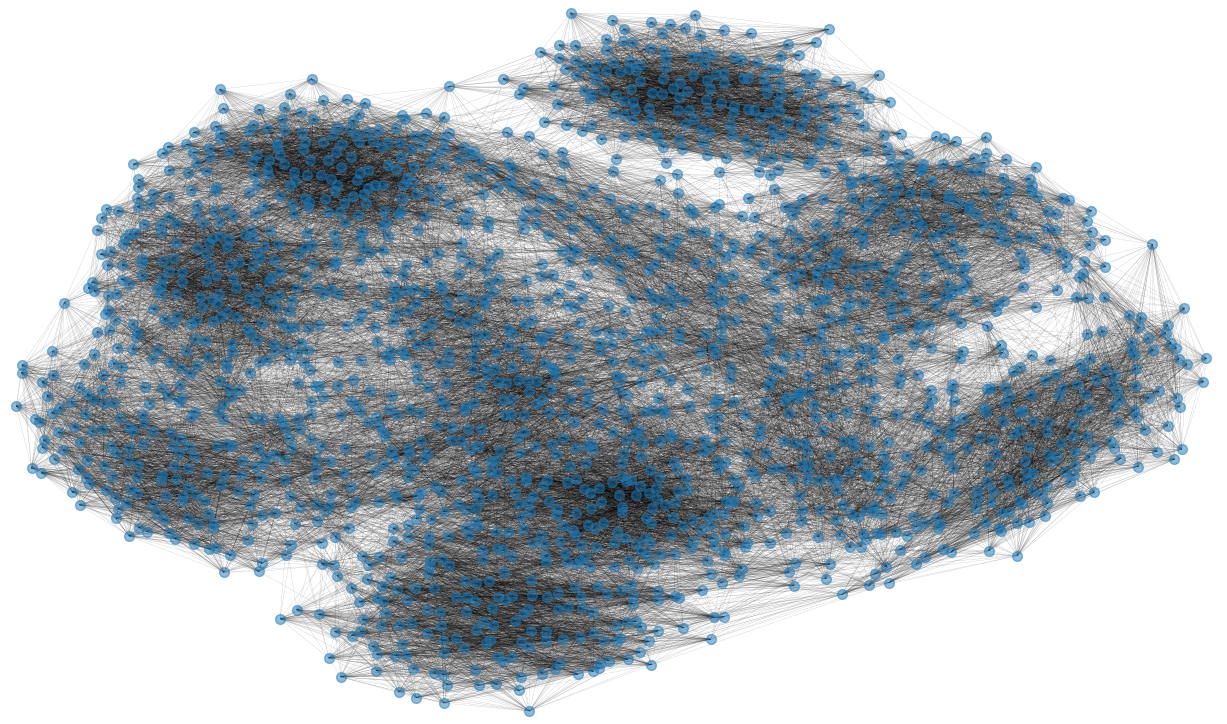
\includegraphics[scale=0.3]{./k-NNG_Kamada_OK.png}
    \caption{grafo k-NN do conjunto de dados de dígitos para $nn = 42$ vizinhos.}
\label{fig:k-NNG}
\end{figure}

A primeira questão que surge no k-médias topológicas é: como construir um grafo a partir de um conjunto de dados multivariado para criar uma aproximação discreta da variedade oculta dos dados? No aprendizado de máquina baseado em grafos, dois métodos populares são particularmente interessantes devido à eficiência computacional \cite{k-NNG,k-NNG2}:

\begin{enumerate}
	\item Grafo k-NN: para cada ponto de dados $\vec{x}_i, i = 1, 2, ..., n$, devemos calcular a distância euclidiana para todas as outras amostras $\vec{x}_j, j \neq i, j = 1, 2, ..., n$. Então, temos que selecionar apenas as $k$ amostras com menor distância (vizinhos mais próximos) e criar uma aresta entre elas.
	\item Grapho $\epsilon$-vizinhos: devemos definir um raio $\epsilon$ e para cada amostra $\vec{x}_i, i = 1, 2, ..., n$ e todas as outras amostras $\vec{x}_j, j \neq i, j = 1, 2, ..., n$, calcule a distância euclidiana entre eles. Para cada ponto dentro da bola de raio $\epsilon$ centrado em $\vec{x}_i$, uma aresta deve ser criada.
\end{enumerate}

Uma segunda questão que surge é: quão bem o comprimento dos caminhos mais curtos em grafos k-NN pode aproximar as verdadeiras distâncias geodésicas subjacentes na variedade oculta dos dados? O Teorema da Convergência Assintótica mostra que, sob certas condições de regularidade, o comprimento dos caminhos mais curtos em grafos k-NN $d_G(\vec{x}_i, \vec{x}_j)$ converge para as distâncias geodésicas $d_M(\vec {x}_i, \vec{x}_j)$ \cite{NIPS2002}. Em resumo, os autores mostram que as duas métricas de distância, $d_G(\vec{x}_i, \vec{x}_j)$ e $d_M(\vec{x}_i, \vec{x}_j)$ aproximam uns aos outros arbitrariamente próximos, já que a densidade dos pontos de dados tende ao infinito. Em resumo, os autores mostram que as duas métricas de distância, $d_G(\vec{x}_i, \vec{x}_j)$ e $d_M(\vec{x}_i, \vec{x}_j)$ aproximam arbitrariamente uma da outra à medida que a densidade dos pontos de dados tende ao infinito.

\vspace{0.5cm}
\begin{theorem}[Teorema da Convergência Assíptica]
	Dado $\lambda_1, \lambda_2, \mu > 0$, mas tão pequenos quanto desejado, então, para uma densidade suficientemente grande de pontos, a seguinte desigualdade é válida:
	\begin{equation}
		1 - \lambda_1 \leq \frac{d_G(\vec{x}_i,\vec{x}_j)}{d_M(\vec{x}_i,\vec{x}_j)} \leq 1 + \lambda_2
    \end{equation} com probabilidade $1 - \mu$, onde $d_G(\vec{x}_i,\vec{x}_j)$ é a distância recuperada (comprimento do caminho mais curto) e $d_M(\vec{x}_i,\vec{x}_j)$ é a verdadeira distância geodésica na variedade oculta dos dados.
\end{theorem}
\vspace{0.5cm}

Os detalhes matemáticos da prova podem ser encontrados no trabalho de Bernstein e colegas \cite{ACT}. A seguir, apresentamos o pseudocódigo para as k-médias topológicas propostas no Algoritmo \ref{topkmeans_algo}.

\begin{algorithm}[H]
\caption{Algoritmo k-means Topologico}\label{topkmeans_algo}
\begin{algorithmic}
\State // Parâmetros:
\State // $X$: a matriz de dados $n \times d$ (cada linha é uma amostra)
\State // $n$: o número de amostras
\State // $k$: o número de clusters
\State // $nn$: o número de vizinhos no grafo k-NN
\Function{Top-k-means}{$X, n, k, nn$}
\State $\vec{s}_1, \vec{s}_2, .., \vec{s}_k \gets select\_random\_seeds(X, k)$ \Comment{Seleciona k centros aleatório}
\State $distances \gets zeros(k, n)$ \Comment{Vetor para armazenar as distancias geodésicas}
\For{$i \gets 1$; $i \leq k$; $i++$}	
	\State $\vec{\mu}_i \gets \vec{s}_i$		
\EndFor
\While{não converge}
	\State $G \gets kNN\_Graph(X, nn)$	\Comment{Construir o grafo k-NN}
	\For{$i \gets 1$; $i \leq k$; $i++$}
		\State $\omega_i \gets \{ \}$		\Comment{Começa com $k$ partições vazias}
	\EndFor
	\For{$j \gets 1$; $i \leq k$; $j++$}
		\State $distances[j] \gets Dijkstra(G, \vec{\mu}_j)$  \Comment{Distâncias geodésicas}
	\EndFor
	\For{$i \gets 1$; $i \leq n$; $i++$}
		\State $j \gets distances[:, i].argmin()$	\Comment{Seleciona o centroide mais próximo}
        \State $\omega_j \gets \omega_j \cup \{ \vec{x}_i \} $	\Comment{Atribui a amostra ao cluster}
	\EndFor
	\For{$i \gets 1$; $i \leq k$; $i++$}
		\State $\vec{\mu}_i \gets \frac{1}{\lvert \omega_i \rvert}\sum_{\vec{x} \in \omega_i} \vec{x}$ \Comment{Recalcula os centroides}
	\EndFor
\EndWhile 
\State \textbf{return} $\omega_1, \omega_2, ..., \omega_k$	
\EndFunction
\end{algorithmic}
\end{algorithm}

Neste ponto, alguns comentários sobre o algoritmo devem ser feitos. Primeiro, observe que, em comparação com k-médias regulares, as k-médias topológicas requerem um parâmetro adicional $nn$, que é o número de vizinhos no grafo k-NN. Alternativamente, pode-se optar por parametrizar o algoritmo em termos de $\epsilon$, que é o raio que define o tamanho da vizinhança (bola centrada em $\vec{x}_i$). Segundo, para construir corretamente o grafo k-NN, ao final de cada iteração, os novos centros devem ser incluídos na matriz de dados $X$, pois muitas vezes eles não pertencem à matriz de dados original. Finalmente, nesta versão do algoritmo, o centro do cluster $\omega_j$ é atualizado calculando a média amostral das amostras atribuídas a ele, mas é possível calcular uma média sobre as distâncias geodésicas, mas isso exigiria outro execução do algoritmo de Dijkstra dentro do loop WHILE. Portanto, para alcançar um equilíbrio entre desempenho e custo computacional, optamos por manter a média amostral.

As principais vantagens das k-médias topológicas propostas sobre as k-médias regulares podem ser resumidas em dois pontos principais:

\begin{itemize}
    \item O K-means normal usa a distância euclidiana, o que significa que é 'cego' para clusters não esféricos e bastante sensível à presença de ruído e valores discrepantes nos dados. Com a incorporação de uma distância geodésica baseada em grafos, pretendemos aliviar essas limitações.
    \item Em espaços de alta dimensão, o poder de discriminação da distância euclidiana é pobre devido à geometria complexa dos hiperespaços. Consequentemente, o desempenho de k-means e outros algoritmos de agrupamento pode ser severamente degradado em conjuntos de dados para os quais o número de recursos $n$ é muito maior que o número de amostras $m$.
\end{itemize}

\subsection{Análise de complexidade}

A complexidade computacional do algoritmo k-means topológico proposto depende das seguintes variáveis: o número de amostras $n$, o número de características $d$, o número de clusters $k$, o número de vizinhos no grafo k-NN $nn$, o número de arestas no grafo k-NN $m$ e o número de iterações $t$, que muitas vezes é desconhecido.

Observe que a definição dos centros iniciais pode ser feita em $O(k)$. A definição da matriz de distâncias é realizada em $O(kn)$, e o loop FOR inicial também é $O(k)$. A análise do loop WHILE principal revela que:

\begin{itemize}
    \item A construção do grafo k-NN pode ser feita em $O(nd~log~n)$ usando uma KD-Tree.
    \item O algoritmo de Dijkstra é executado $k$ vezes por iteração, resultando em um custo total de $O(km~log~n)$.
    \item O loop FOR de atribuição de rótulo custou $O(kn)$.
    \item O cálculo dos novos centros custou $O(nd)$, como na partição $\omega_1 + \omega_2 + ... + \omega_k = n$.
\end{itemize}

Como o loop WHILE principal é executado um número desconhecido de iterações $t$, o custo total do k-médias topológico é:

\begin{align}
	T(n) & = O(kn) + O(tnd~log~n) + O(tkm~log~n) + O(tkn) + O(tnd) \\ \nonumber
	     & = O(tnd~log~n) + O(tkm~log~n) = O(t(nd+km)log~n)
\end{align}

Portanto, o K-means topológico depende linear e logaritmicamente ao número de amostras $n$ e linearmente ao número de arestas do grafo k-NN $m$, que em termos de complexidade computacional é considerado um algoritmo bastante eficiente.

\section{Experimentos e resultados}

A fim de testar e avaliar o desempenho do método proposto em relação a k-means regular. Foram selecionados algumas métricas de avaliação de cluster (índices externos) para avaliar o desempenho dos algoritmos:  Rand index \cite{Rand1,Rand2}, mutual information score \cite{Mutual}, (V-measure, completeness, homogeneity) \cite{Vmeasure}, Fowlkes-Mallows \cite{Fowlkes}, Silhouettes \cite{Silhouettes}, Calinski-Harabasz \cite{Calinski} e Davies-Bouldin \cite{Davies}.

O primeiro conjunto de experimentos foi projetado para comparar o desempenho dos métodos em conjuntos de dados reais de alta dimensionalidade. Todos os conjuntos de dados selecionados estão disponíveis gratuitamente no repositório \url{www.openml.org}. A Tabela \ref{tab:data} descreve cada conjunto de dados com nomes, número de amostras $n$, número de características $m$ e número de classes $k$. Note que a maioria dos conjuntos de dados contém dados de microarranjo do projeto GEMLeR. Este projeto fornece uma coleção de conjuntos de dados de expressão gênica que podem ser usados para avaliar algoritmos de aprendizado de máquina orientados à expressão gênica. Eles podem ser usados para estimar diferentes métricas de qualidade (por exemplo, acurácia, precisão, área sob a curva ROC, etc.) para algoritmos de classificação, seleção de características ou clustering. Cada amostra de expressão gênica no repositório GEMLeR vem de um grande repositório público expO (Expression Project For Oncology) do International Genomics Consortium \cite{GEMLeR}.

\begin{table}[htb]
%%% Generated by mktable on Sat Dec 27 16:38:40 2008
%%% Started by papa with args: mktable accuracies.txt
\centering
\caption{Número de amostras, recursos e classes dos conjuntos de dados openML selecionados para o primeiro conjunto de experimentos.}
\begin{tabular}{ccccc}
\toprule
\textbf{Numero} & \textbf{Conjunto de Dados}  & \textbf{\# Amostras} & \textbf{\# Atributos} & \textbf{\# Classes} \\
\midrule
1  & micro-mass                        & 360   & 1300    & 10 \\
2  & monks-problems-1                  & 556   & 6       & 2  \\
3  & breast-tissue                     & 106   & 9       & 6  \\
4  & GCM                               & 190   & 16063   & 14 \\
5  & balance-scale                     & 625   & 4       & 3  \\
6  & servo                             & 167   & 4       & 2  \\
7  & AP\_Prostate\_Uterus              & 193   & 10935   & 2  \\
8  & AP\_Colon\_Kidney                 & 546   & 10935   & 2  \\
9  & AP\_Breast\_Kidney                & 604   & 10935   & 2  \\
10 & AP\_Breast\_Ovary                 & 542   & 10935   & 2  \\
11 & AP\_Breast\_Colon                 & 630   & 10935   & 2  \\
12 & leukemia                          & 72    & 7129    & 2  \\
13 & hepatitisC                        & 283   & 54621   & 3  \\
14 & Ovarian                           & 253   & 15154   & 2  \\
15 & SRBCT                             & 83    & 2308    & 4  \\
17 & Colon                             & 62    & 2000    & 2  \\
17 & climate-model-simulation-crashes  & 540   & 20      & 2  \\
18 & pasture                           & 36    & 22      & 3  \\
19 & glass                             & 214   & 9       & 6  \\
20 & kc1-binary                        & 145   & 94      & 2  \\
21 & dermatology                       & 366   & 34      & 6  \\
22 & backache                          & 180   & 31      & 2  \\
23 & lsvt                              & 126   & 310     & 2  \\
24 & thoracic-surgery                  & 470   & 16      & 2  \\
25 & planning-relax                    & 182   & 12      & 2  \\
26 & tr31.wc                           & 927   & 10128   & 7  \\
27 & tr45.wc                           & 690   & 8261    & 10 \\
\bottomrule  
\end{tabular}
\label{tab:data}
\end{table}

É possível notar que uma característica comum à maioria dos conjuntos de dados é que o número de atributos $m$ é muito maior que o número de amostras $n$. Por exemplo, no conjunto de dados número 7, AP\_Prostate\_Uterus, o número de características é mais de 56 vezes o número de amostras, uma situação que representa um difícil desafio para algoritmos de agrupamento. %Figure \ref{fig:AP} shows an illustration of the k-NN graph for this dataset, considering the parameter $nn = 14$ (number of neighbors). Note that the lack of a cluster structure is evident from the k-NN graph, indicating a complex problem.

%\begin{figure}
%	\centering
%	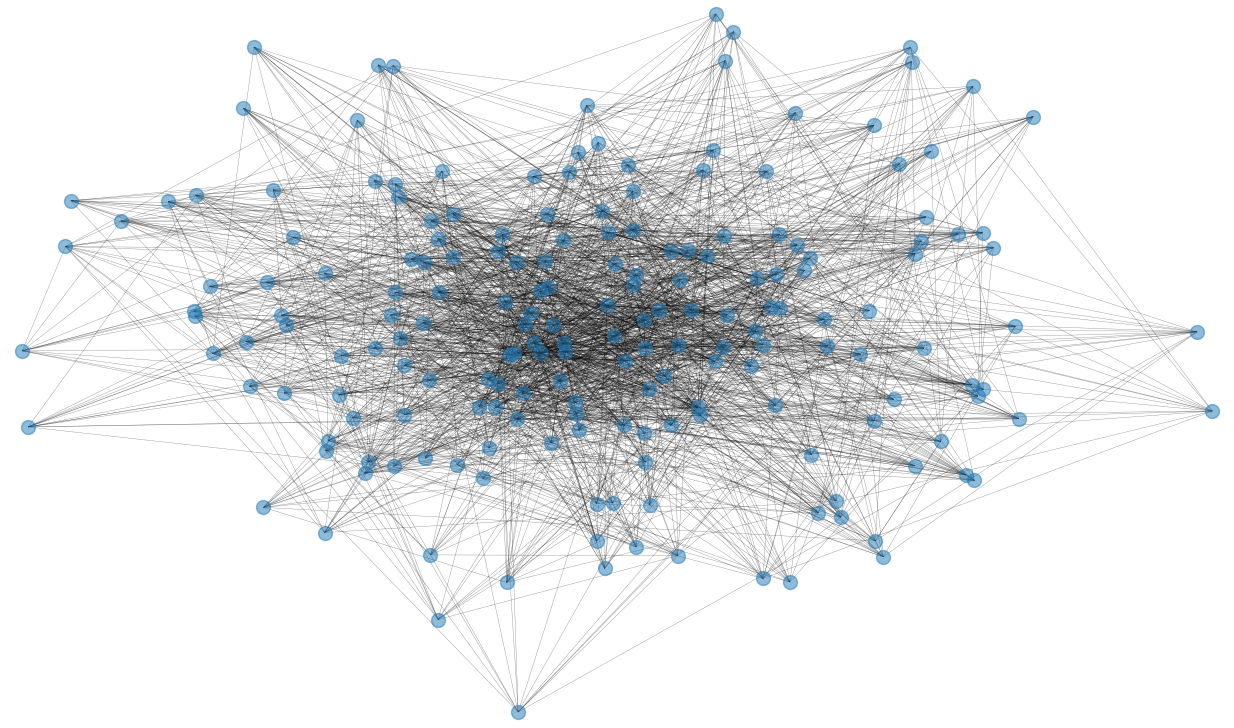
\includegraphics[scale=0.3]{./AP_Graph_OK.png}
%    \caption{k-NN graph of the AP\_Prostate\_Uterus dataset for $nn = 14$ neighbors.}
%\label{fig:AP}
%\end{figure}

Os resultados quantitativos para os algoritmos de agrupamento são apresentados na Tabela \ref{tab:restopk} referentes ao k-means topológico e na Tabela \ref{tab:reskmeans} referentes ao k-means regular.

\begin{table}[ht]
    \centering
    \footnotesize
    \setlength{\tabcolsep}{4pt}
    \caption{Metricas usando o algoritmo de kmeans topológico.}
    \begin{tabular}{@{}p{0.1cm}p{2.3cm}p{1.3cm}p{1cm}p{1cm}p{0.8cm}p{1cm}p{1cm}p{0.8cm}p{1cm}p{1cm}p{0.8cm}@{}}
        \toprule
        \textbf{\#} & 
        \textbf{Nome} & 
        \textbf{Complet.} & 
        \textbf{F. Mallows} & 
        \textbf{Homog.} & 
        \textbf{V Meas.} & 
        \textbf{Adj. Rand} & 
        \textbf{NMI} & 
        \textbf{Silh.} & 
        \textbf{C. Harab.} & 
        \textbf{D. Bouldin} & 
        \textbf{Tempo} \\
        \midrule
        1 & micro-mass & 0.6 & 0.44 & 0.55 & 0.58 & 0.35 & 0.6 & 0.2 & 86.58 & 1.34 & 125.87 \\
        2 & monks-problems-1 & 0.08 & 0.56 & 0.08 & 0.08 & 0.1 & 0.08 & 0.19 & 154.83 & 1.8 & 6.33 \\
        3 & breast-tissue & 0.18 & 0.24 & 0.17 & 0.18 & 0.08 & 0.18 & 0.22 & 23.45 & 1.37 & 0.72 \\
        4 & GCM & 0.44 & 0.3 & 0.41 & 0.43 & 0.23 & 0.43 & 0.19 & 54.24 & 1.28 & 594.42 \\
        5 & balance-scale & 0.12 & 0.48 & 0.13 & 0.12 & 0.14 & 0.12 & 0.12 & 102.36 & 1.95 & 1.12 \\
        6 & servo & 0.04 & 0.59 & 0.04 & 0.04 & 0.03 & 0.04 & 0.2 & 44.9 & 1.7 & 1.73 \\
        7 & AP\_Colon\_Kidney & 0.11 & 0.58 & 0.1 & 0.1 & 0.1 & 0.1 & 0.15 & 85.36 & 2.18 & 89.54 \\
        8 & AP\_Breast\_Kidney & 0.11 & 0.59 & 0.1 & 0.1 & 0.11 & 0.1 & 0.13 & 88.50 & 2.25 & 97.11 \\
        9 & AP\_Breast\_Ovary & 0.01 & 0.58 & 0.004 & 0.004 & 0.01 & 0.004 & 0.25 & 80.75 & 1.77 & 91.47 \\
        10 & AP\_Breast\_Colon & 0.01 & 0.54 & 0.01 & 0.01 & 0.012 & 0.01 & 0.18 & 134.51 & 1.9 & 94.03 \\
        11 & AP\_Prostate\_Uterus & 0.17 & 0.61 & 0.16 & 0.17 & 0.15 & 0.17 & 0.16 & 38.05 & 1.92 & 50.27 \\
        12 & leukemia & 0.05 & 0.58 & 0.03 & 0.04 & 0.03 & 0.04 & 0.17 & 12.26 & 1.77 & 2.32 \\
        13 & hepatitisC & 0.15 & 0.65 & 0.22 & 0.17 & 0.09 & 0.17 & -0.003 & 13.53 & 2.94 & 166.31 \\
        14 & Ovarian & 0.007 & 0.54 & 0.007 & 0.007 & 0.004 & 0.007 & 0.17 & 56.41 & 1.88 & 56.41 \\
        15 & SRBCT & 0.14 & 0.34 & 0.11 & 0.12 & 0.04 & 0.12 & 0.10 & 10.49 & 1.69 & 3.46 \\
        16 & Colon & 0.02 & 0.56 & 0.02 & 0.02 & 0.001 & 0.02 & 0.151 & 9.33 & 1.92 & 2.24 \\
        17 & climate... & 0.06 & 0.65 & 0.15 & 0.09 & 0.01 & 0.09 & 0.54 & 1126.12 & 0.62 & 4.03 \\
        18 & pasture & 0.23 & 0.45 & 0.2 & 0.21 & 0.15 & 0.21 & 0.49 & 231.73 & 1.36 & 0.83 \\
        19 & glass & 0.22 & 0.33 & 0.25 & 0.24 & 0.13 & 0.23 & 0.22 & 95.99 & 1.14 & 2.63 \\
        20 & kc1-binary & 0.15 & 0.61 & 0.15 & 0.15 & 0.2 & 0.15 & 0.46 & 36.51 & 0.79 & 1.55 \\
        21 & dermatology & 0.15 & 0.24 & 0.15 & 0.15 & 0.06 & 0.15 & 0.29 & 516.92 & 1.11 & 18.14 \\
        22 & backache & 0.01 & 0.63 & 0.01 & 0.01 & -0.006 & 0.01 & 0.41 & 184.8 & 0.82 & 2.36 \\
        23 & lsvt & 0.02 & 0.54 & 0.02 & 0.02 & -0.01 & 0.02 & 0.63 & 227.9 & 0.53 & 2.91 \\
        24 & thoracic-surgery & 0.003 & 0.69 & 0.002 & 0.002 & -0.007 & 0.002 & 0.57 & 430.68 & 0.71 & 4.03 \\
        25 & planning-relax & 0.002 & 0.58 & 0.002 & 0.002 & 0.003 & 0.002 & 0.15 & 32.72 & 1.93 & 0.88 \\
        26 & tr31.wc & 0.2 & 0.38 & 0.18 & 0.19 & 0.12 & 0.19 & -0.01 & 565.44 & 2.45 & 1825.38 \\
        27 & tr45.wc & 0.26 & 0.25 & 0.21 & 0.23 & 0.08 & 0.23 & -0.02 & 140.28 & 2.35 & 836.54 \\
        \midrule
        28 & \textbf{Media} & 0.13 & 0.5 & 0.13 & 0.13 & 0.08 & 0.13 & 0.23 & 169.81 & 1.61 & 151.213 \\
        29 & \textbf{Desvio padrão} & 0.14 & 0.14 & 0.13 & 0.13 & 0.09  & 0.13 & 0.17 & 242.22 & 0.6 & 384.91 \\
        30 & \textbf{Máximo} & 0.61 & 0.69 & 0.55 & 0.58 & 0.35 & 0.58 & 0.63 & 1126.12 & 2.94 & 1825.38 \\
        \bottomrule
    \end{tabular}
    \label{tab:restopk}
\end{table}

\begin{table}[ht]
    \centering
    \footnotesize
    \setlength{\tabcolsep}{4pt}
    \caption{Metricas usando o algoritmo de kmeans padrão.}
    \begin{tabular}{@{}p{0.1cm}p{2.3cm}p{1.3cm}p{1cm}p{1cm}p{0.8cm}p{1cm}p{1cm}p{0.8cm}p{1cm}p{1cm}p{0.8cm}@{}}
        \toprule
        \textbf{\#} & 
        \textbf{Nome} & 
        \textbf{Complet.} & 
        \textbf{F. Mallows} & 
        \textbf{Homog.} & 
        \textbf{V Meas.} & 
        \textbf{Adj. Rand} & 
        \textbf{NMI} & 
        \textbf{Silh.} & 
        \textbf{C. Harab.} & 
        \textbf{D. Bouldin} & 
        \textbf{Tempo} \\
        \midrule
        1 & micro-mass & 0.7 & 0.48 & 0.60 & 0.65 & 0.38 & 0.65 & 0.24 & 88.81 & 1.27 & 4.2\\
        2 & monks-problems-1 & 0.08 & 0.55 & 0.08 & 0.08 & 0.10 & 0.08 & 0.23 & 202.32 & 1.63 & 3.17\\
        3 & breast-tissue & 0.20 & 0.25 & 0.2 & 0.20 & 0.1 & 0.2 & 0.14 & 13.31 & 1.75 & 0.28\\
        4 & GCM & 0.49 & 0.29 & 0.45 & 0.47 & 0.22 & 0.47 & 0.11 & 26.75 & 1.82 & 20.29\\
        5 & balance-scale & 0.1 & 0.46 & 0.13 & 0.11 & 0.13 & 0.11 & 0.17 & 136.76 & 1.69 & 3.23\\
        6 & servo & 0.14 & 0.59 & 0.16 & 0.15 & -0.06 & 0.15 & 0.30 & 69.35 & 1.33 & 0.26\\
        7 & AP\_Colon\_Kidney & 0.006 & 0.50 & 0.006 & 0.006 & 0.005 & 0.006 & 0.16 & 105.26 & 2.19 & 18.71\\
        8 & AP\_Breast\_Kidney & 0.005 & 0.51 & 0.005 & 0.005 & 0.009 & 0.005 & 0.15 & 108.48 & 2.25 & 20.9\\
        9 & AP\_Breast\_Ovary & 0.11 & 0.69 & 0.003 & 0.005 & 0.005 & 0.005 & 0.79 & 577.22 & 0.43 & 16.61\\
        10 & AP\_Breast\_Colon & 0.01 & 0.51 & 0.01 & 0.01 & 0.01 & 0.01 & 0.18 & 151.04 & 1.96 & 18.53\\
        11 & AP\_Prostate\_Uterus & 0.03 & 0.53 & 0.03 & 0.03 & 0.03 & 0.03 & 0.16 & 45.03 & 1.98 & 7.99\\
        12 & leukemia & 0.008 & 0.54 & 0.007 & 0.007 & 0.01 & 0.007 & 0.12 & 9.32 & 2.56 & 2.96\\
        13 & hepatitisC & 0.15 & 0.62 & 0.31 & 0.2 & 0.14 & 0.2 & 0.06 & 16.46 & 3.37 & 80.17\\
        14 & Ovarian & 0.007 & 0.52 & 0.007 & 0.007 & 0.009 & 0.007 & 0.19 & 69.71 & 1.82 & 23.51\\
        15 & SRBCT & 0.21 & 0.35 & 0.19 & 0.2 & 0.08 & 0.2 & 0.09 & 7.05 & 2.4 & 2.03\\
        16 & Colon & 0.01 & 0.52 & 0.01 & 0.01 & -0.007 & 0.01 & 0.09 & 7.68 & 2.7 & 1.39\\
        17 & climate...& 0.06 & 0.65 & 0.16 & 0.09 & 0.02 & 0.09 & 0.54 & 1118.47 & 0.64 & 3.18\\
        18 & pasture & 0.42 & 0.57 & 0.42 & 0.42 & 0.37 & 0.42 & 0.5 & 104.87 & 0.65 & 0.24\\
        19 & glass & 0.45 & 0.50 & 0.38 & 0.41 & 0.26 & 0.41 & 0.44 & 122.29 & 0.94 & 0.31\\
        20 & kc1-binary & 0.14 & 0.69 & 0.04 & 0.06 & 0.04 & 0.06 & 0.86 & 181.8 & 0.59 & 0.88\\
        21 & dermatology & 0.09 & 0.21 & 0.09 & 0.09 & 0.02 & 0.09 & 0.27 & 509.18 & 1.1 & 2.92\\
        22 & backache & 0.01 & 0.63 & 0.01 & 0.01 & -0.03 & 0.01 & 0.42 & 185.1 & 0.86 & 0.29\\
        23 & lsvt & 0.02 & 0.61 & 0.017 & 0.02 & -0.03 & 0.02 & 0.71 & 281.44 & 0.47 & 1.43\\
        24 & thoracic-surgery & 0.005 & 0.78 & 0.002 & 0.002 & -0.017 & 0.002 & 0.74 & 641.0 & 0.42 & 3.09\\
        25 & planning-relax & 0.0 & 0.54 & 0.0 & 0.0 & -0.004 & 0.0 & 0.16 & 38.16 & 2.04 & 0.29\\
        26 & tr31.wc & 0.23 & 0.48 & 0.05 & 0.09 & 0.04 & 0.09 & 0.66 & 1740.9 & 1.20 & 39.31\\
        27 & tr45.wc & 0.28 & 0.31 & 0.09 & 0.14 & 0.007 & 0.14 & 0.26 & 314.31 & 1.57 & 32\\
        \midrule
        28 & \textbf{Media} & 0.15 & 0.51 & 0.13 & 0.13 & 0.07 & 0.13 & 0.32 & 254.52 & 1.54 & 11.41 \\
        29 & \textbf{Desvio padrão} & 0.18 & 0.13 & 0.16 & 0.17 & 0.11  & 0.17 & 0.24 & 389.02 & 0.77 & 17.53 \\
        30 & \textbf{Máximo} & 0.7 & 0.78 & 0.6 & 0.65 & 0.38 & 0.65 & 0.86 & 1,740.9 & 3.37 & 80.17 \\
        \bottomrule
    \end{tabular}
    \label{tab:reskmeans}
\end{table}

Observando os resultados, vemos que, para esses conjuntos de dados, algumas metricas do k-médias topológicas propostas superam as k-médias padrão. Em todos os experimentos, o parâmetro $k$ (número de clusters) é igual ao número de classes e o número de vizinhos $nn$ é definido como $\lfloor \sqrt{n} \rfloor$. Para gerar os resultados, calculamos o desempenho médio após 30 inicializações aleatórias de k-médias e k-médias topológicas. Para verificar se as diferenças são significativas, foi realizado um teste não paramétrico de Wilcoxon. De acordo com o teste, para um nível de significância $\alpha = 0,05$, há fortes evidências de que as k-médias topológicas propostas tiveram melhor desempenho do que as k-médias regulares em termos de índice Rand ($p < 0,001$), informação mútua normalizada ( $p < 0,001$) e medida V ($p < 0,001$).

Alguns comentários sobre as k-médias topológicas devem ser abordados neste ponto. Um aspecto importante do método proposto é que devemos garantir que o o k-NN esteja conectado, de forma a permitir que os centros se movam livremente em torno de todo o conjunto de vértices. Caso contrário, se a inicialização aleatória escolher todos os centróides para estarem em um único componente conectado, o algoritmo nunca rotulará as amostras que pertencem a outros componentes conectados de $G$. Existem duas estratégias para garantir que $G$ esteja conectado: 1) defina o número de vizinhos $nn = \lfloor \sqrt{n} \rfloor$ e enquanto $G$ não estiver conectado, incremente $nn$ em um e construa um novo  k-NN; e 2) começar com um  completo, extrair a árvore geradora mínima (MST) e adicionar as arestas do MST ao grafo k-NN construído usando $nn = \lfloor \sqrt{n} \rfloor$. Alguns autores argumentam que em vez da raiz quadrada do número de amostras, uma boa estimativa para o número de vizinhos é o logaritmo de base dois do número de amostras \cite{RandomGraphs,LOG}. No entanto, em nossos experimentos, $nn = log_2~n$ produziu grafos desconectados para vários conjuntos de dados de alta dimensão, então optamos por considerar a configuração de parâmetro padrão como $nn = \lfloor \sqrt{n} \rfloor$.

As principais desvantagens das k-médias topológicas propostas ainda estão relacionadas às limitações do k-means normal. Primeiro, o esquema de inicialização aleatória: o desempenho do algoritmo está diretamente relacionado à seleção aleatória dos centróides iniciais, algo que não está sob controle. Melhores estratégias de inicialização para k-means podem ser adaptadas para k-means topológicos, como k-means++ por exemplo \cite{kmeans++}. Métodos baseados em propriedades topológicas do grafo k-NN também podem ser empregados para esse fim. Outra questão está relacionada à definição do número de clusters $k$. Em k-médias topológicas é possível evitar a dependência do parâmetro $k$ estimando seu valor através de um algoritmo de detecção de comunidade no grafo k-NN \cite{Community}.

\section{Conclusões e observações finais}

Algoritmos de clustering são ferramentas versáteis em aprendizado de máquina, contribuindo para vários aspectos de análise, exploração e compreensão de dados. Suas aplicações abrangem diferentes domínios, tornando-as indispensáveis para pesquisadores, cientistas de dados e analistas que buscam descobrir padrões e estruturas em dados complexos. Esses algoritmos desempenham um papel crucial no aprendizado de máquina, especialmente no aprendizado não supervisionado. Alguns exemplos de problemas onde o agrupamento desempenha um papel importante são: descoberta e reconhecimento de padrões, exploração e compreensão de dados, detecção de anomalias, processamento de imagens e sinais, redução de dimensionalidade, sistemas de recomendação, análise de documentos, bioinformática e na redução da carga de rotulagem.

No entanto, agrupar dados de alta dimensão ainda é uma tarefa desafiadora, especialmente em problemas de tamanho amostral pequeno. Parte desta complexidade vem das propriedades geométricas dos hiperespaços, ou seja, espaços com milhares de dimensões. Dados de alta dimensão representam desafios devido à maldição da dimensionalidade porque as métricas de distância tradicionais, como a distância euclidiana, podem tornar-se menos significativas, afetando negativamente o desempenho dos algoritmos de agrupamento.

Neste artigo, propusemos um algoritmo topológico k-means que utiliza caminho ótimo em grafos para aproximar as verdadeiras distâncias geodésicas na variedade de dados. Em resumo, a motivação para k-means topológicos foi melhorar a capacidade do k-means de lidar com dados de alta dimensão. No geral, as principais contribuições do método proposto estão diretamente relacionadas com a mitigação da cegueira do agrupamento não esférico de k-médias regulares. Nossos resultados mostraram que k-means topológicos são capazes de produzir clusters melhores que k-means nomal. Apesar de ser um algoritmo viável e promissor, o k-means topológico não é perfeito e possui limitações. O mais destacado é que o desempenho depende de uma boa escolha inicial de centróides, que na maioria das vezes não está sob controle, além de um leve aumento no tempo computacional.

A fim de superar as limitações topológicas de k-means, trabalhos futuros podem incluir o desenvolvimento de melhores estratégias de inicialização, como a heurística kmeans++ e um método baseado em curvatura para amostragem de dados baseado no operador de forma. Outra melhoria futura diz respeito à determinação automática do número de clusters por meio da detecção de comunidades no grafo k-NN. Outras estratégias para construção de grafos podem ser adotadas como forma de tornar mais evidente a estrutura subjacente do cluster nos dados, facilitando o trabalho das k-médias topológicas. Finalmente, o uso de diferentes métricas para ponderar as arestas do grafo k-NN pode ser interessante para melhorar a capacidade topológica de k-médias de aprender diferentes formas de clusters.

%%===========================================================================================%%
%% If you are submitting to one of the Nature Portfolio journals, using the eJP submission   %%
%% system, please include the references within the manuscript file itself. You may do this  %%
%% by copying the reference list from your .bbl file, paste it into the main manuscript .tex %%
%% file, and delete the associated \verb+\bibliography+ commands.                            %%
%%===========================================================================================%%

\bibliography{bibliography}% common bib file
%% if required, the content of .bbl file can be included here once bbl is generated
%%\input sn-article.bbl


\end{document}

